\chapter{Human Driver Modelling}
\label{sec:human_driver}

In this chapter, the human driver model that Salvucci presents in \cite{salvucci_1} is implemented and the metrics used to verify the model are established. Initially, the model is implemented in \textit{Matlab} based on the integrated driver model. To be able to verify it using the probabilistic model checking techniques presented in Chapter 2, the model undergoes an abstraction process, out of which a discrete-time Markov chain is obtained using several different approaches and assumptions. Metrics are then established to be able to evaluate whether the model meets the requirements and how well the human performs in a given situation. Finally, a simulator is presented in Section~\ref{sec:simulator} in order to allow visualisation of paths in the model.

\section{Continuous Driver Model using ACT-R}

In order to obtain a continuous driver model, we interpret Salvucci's integrated driver model as presented in \cite{salvucci_1}. The scenario considered is the one Salvucci envisioned: a multilane highway with moderate (or low) traffic \cite{salvucci_1}. The model uses the three modules presented in Figure~\ref{fig:high_level_salvucci}, that is, monitoring, decision making and control. All these modules rely on the constant update of the environment, as some are based on visual or low-level perception cues. While the human model is presented clearly in \cite{salvucci_1}, the dynamics of the car (which is part of the environment) are left to the reader, as it is outside the scope of the paper. In that sense, some assumptions had to be made about the environment.

The main initial assumption is that the driver is perfectly aware of its surroundings, and thus it is able to obtain the positions of other vehicles (within a certain distance) and the near and far points perfectly (this assumption is challenged later in the abstraction process). Additionally, the environment is assumed to change at the same rate as a cycle of the ACT-R model.

The overall view of the system is presented in Figure~\ref{fig:driver_model_overview}. The information flow is marked using the dotted arrows, while the sequential flow of the program is marked in the filled, lighter gray ones. Both the monitoring and the decision making make use of the perception which corresponds to querying the environment for the information (e.g. near and far point or another vehicle's position). The control both queries and sends updated information (e.g. vehicle position, velocity and acceleration) to the environment. Modules are updated sequentially, following the order: control, monitoring, decision making and environment (e.g. position, velocity and acceleration of other vehicles).

\vspace{1em}
\begin{figure}[h]
    \centering
    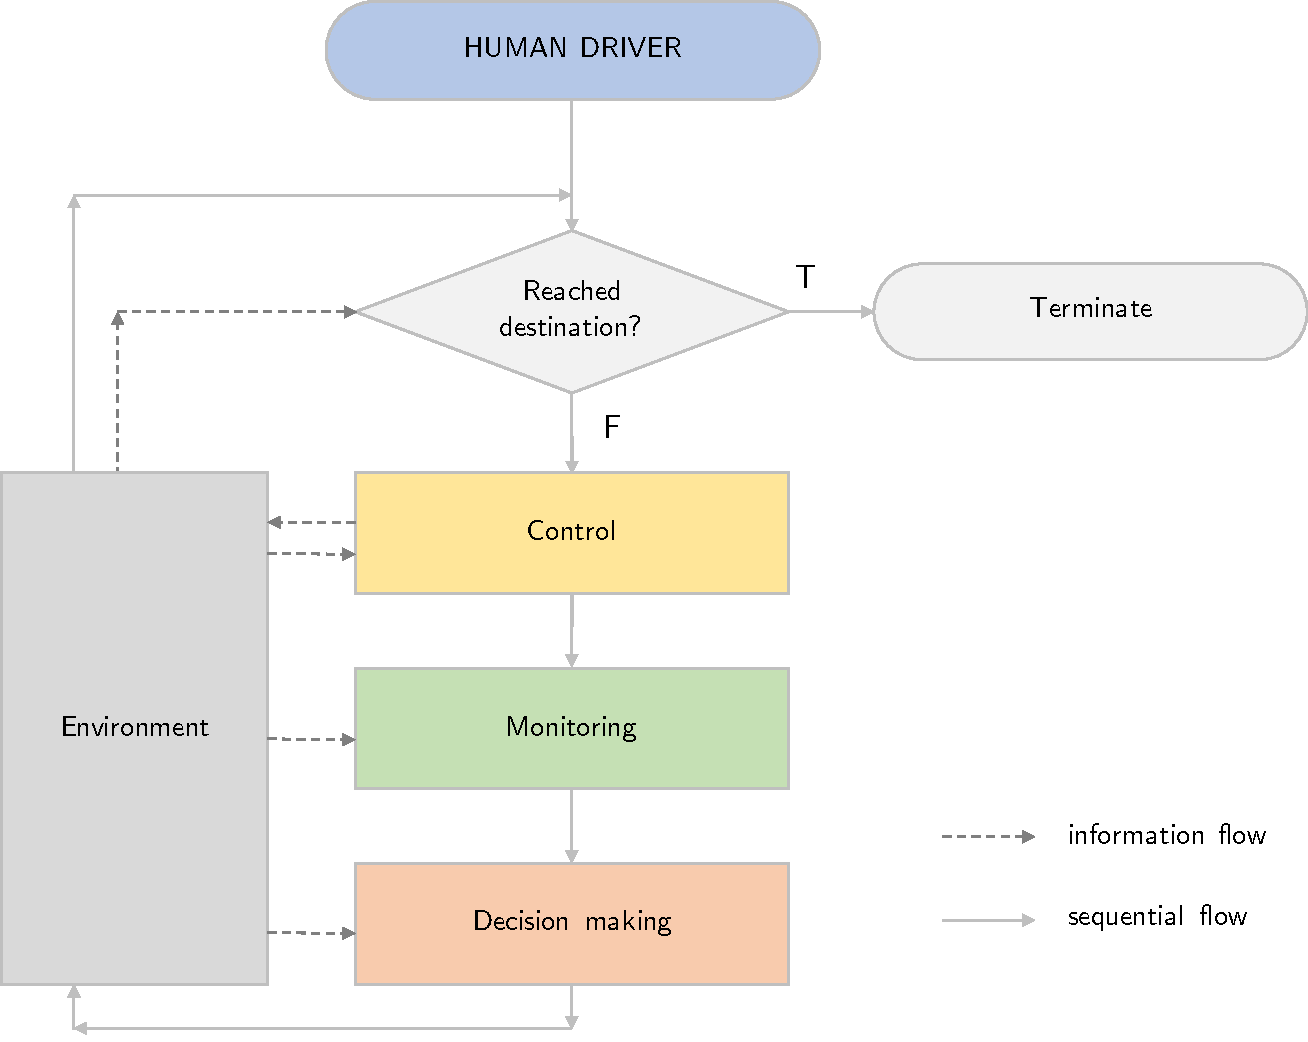
\includegraphics[width=0.85\textwidth]{matlab.pdf}
    \caption{Continuous Driver Model overview.}
    \label{fig:driver_model_overview}
\end{figure}

The monitoring module is implemented according to the flowchart presented in Figure~\ref{fig:monitor}, from the description given in \cite{salvucci_1}. The threshold for monitoring is set at $0.2$, as this is the value suggested by Salvucci in \cite{salvucci_1}. The output of this process corresponds to altering the global variable $a$ corresponding to the declarative memory cell composed of $k$ chunks. No specific value for $k$ is given by Salvucci in \cite{salvucci_1}, but it is taken to be 8 from \cite{lam}. The function \texttt{GET\_DISTANCE} is not described in depth due to the fact that it is trivial under the assumption stated previously.

The overall flowchart of the decision making module is shown in Figure~\ref{fig:dm}. The high level part is similar to the flowchart presented in Figure~\ref{fig:flowchart_dm}, with small differences related to the loading of variables and information from the different memories available. It is worth noticing that the control makes use of the function \texttt{LOOK\_VEHICLE} initially presented in the monitoring module to verify the presence of a vehicle in a relative position of a lane. The flow of the function \texttt{SET\_LANE\_FOLLOWING} is also omitted due to the trivial nature of this function under the assumptions made.

Finally, a flowchart for the control module is presented in Figure~\ref{fig:control}. This module is responsible for the calculation of $\Delta\varphi(t)$ and $\Delta\psi(t)$ and the update of the position. Given these two values, the position is updated following discrete laws of motion applied to rigid objects, particularly:

\begin{equation}
\begin{aligned}
	& \mathbf{v}(t) = \mathbf{v}(t-1) + \mathbf{a}(t)\Delta t\\
	& \mathbf{x}(t) = \mathbf{x}(t-1) + \mathbf{v}(t-1)\Delta t + \frac{1}{2}  \mathbf{a}(t)\Delta t^2 \\
	& t = t + \Delta t
\end{aligned}
\end{equation}

where $\mathbf{x}(t) = (x(t), y(t))$, $\mathbf{v}(t) = (v_x(t), v_y(t))$, and $\mathbf{a}(t) = (a_x(t), a_y(t))$, with:

\begin{equation}
\begin{aligned}
	a_x(t) & = \Delta\psi(t) \\
	a_y(t) & = \sin(\Delta\varphi(t))
\end{aligned}
\end{equation}

\begin{figure}
\centering
\begin{subfigure}{1\textwidth}
  \centering
  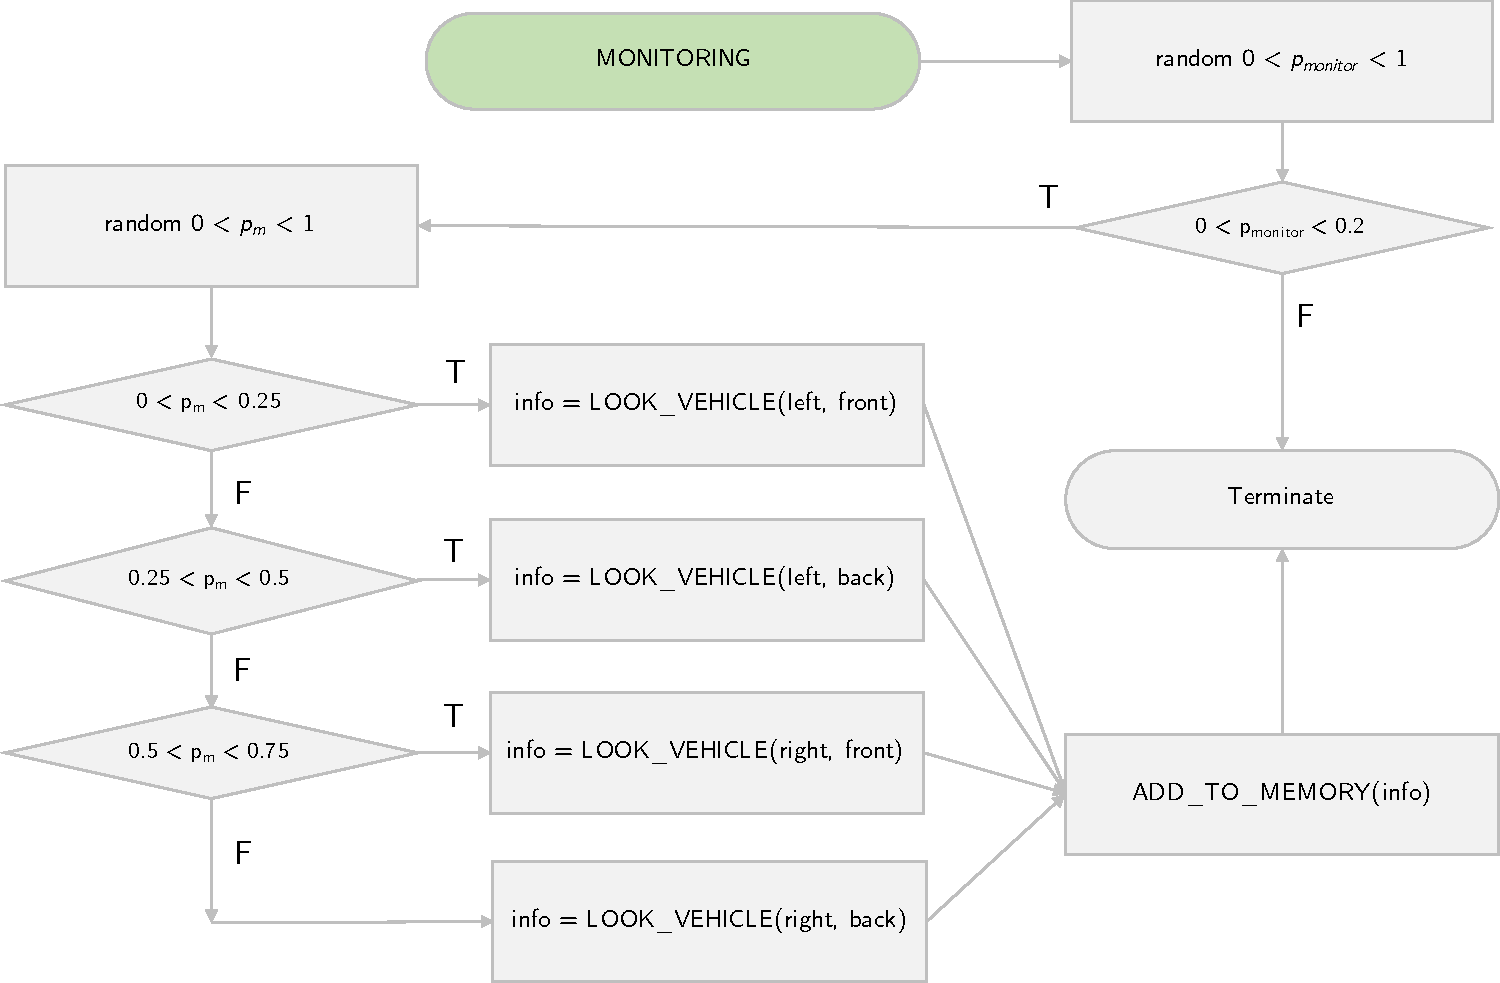
\includegraphics[width=1\textwidth]{monitor_1.pdf}
\end{subfigure}\\ \vspace{2em}
\begin{subfigure}{1\textwidth}
  \centering
  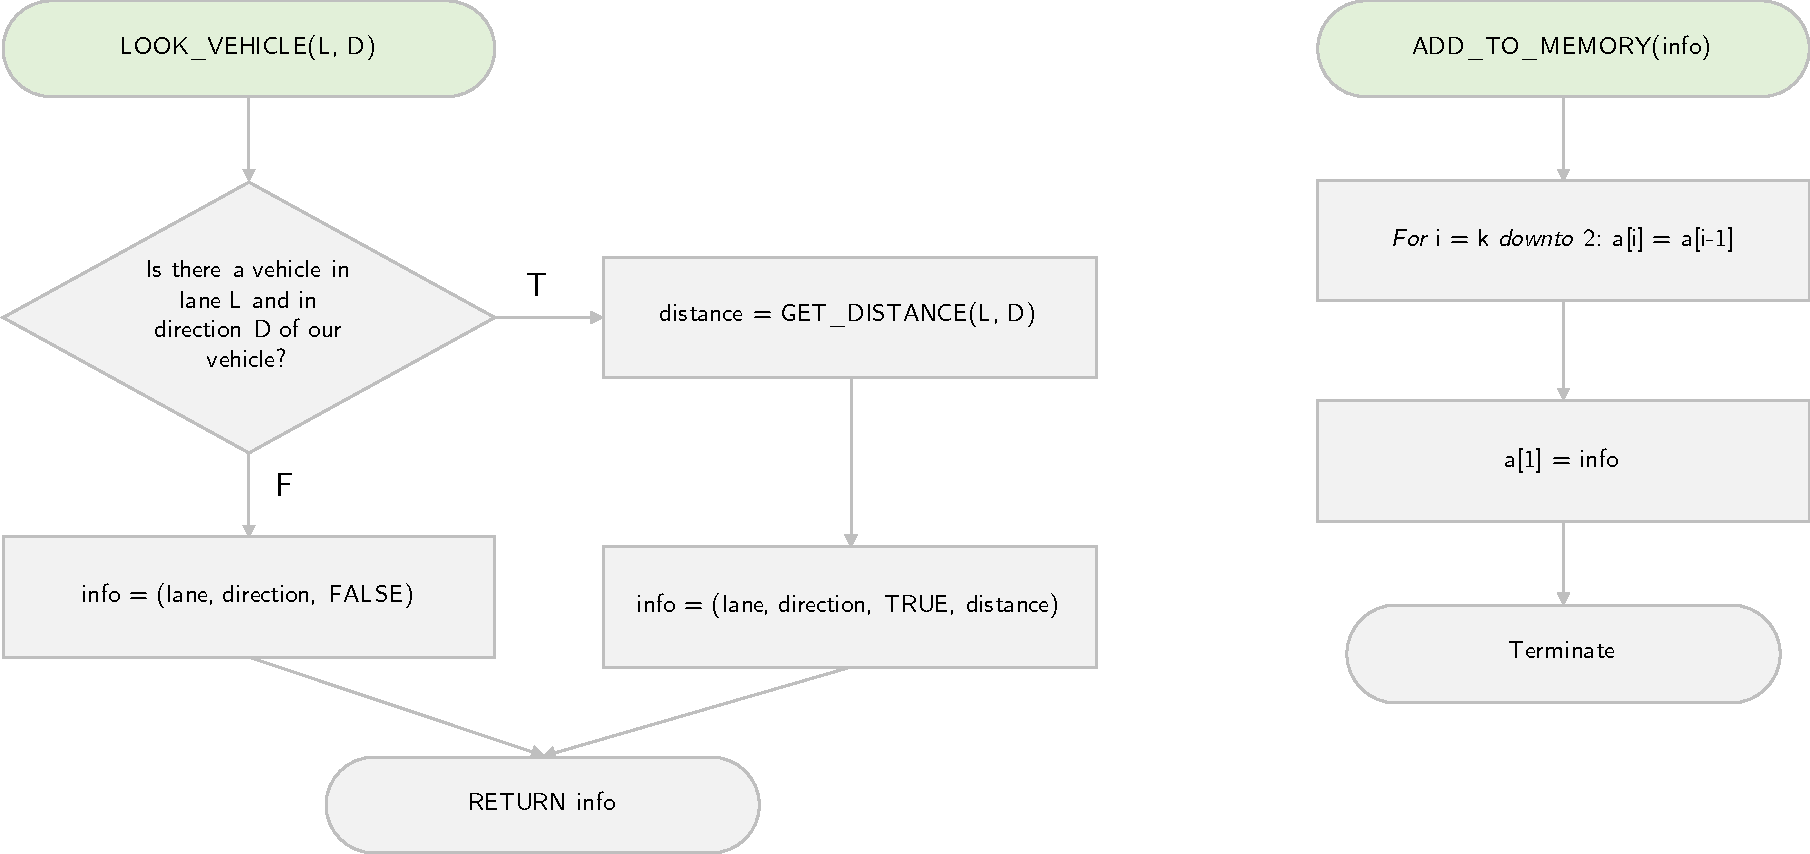
\includegraphics[width=1\linewidth]{monitor_2.pdf}
\end{subfigure} \vspace{2em}
\caption{Flowchart of the Monitoring module.}
\label{fig:monitor}
\end{figure}

\begin{figure}
\centering
\begin{subfigure}{1\textwidth}
  \centering
  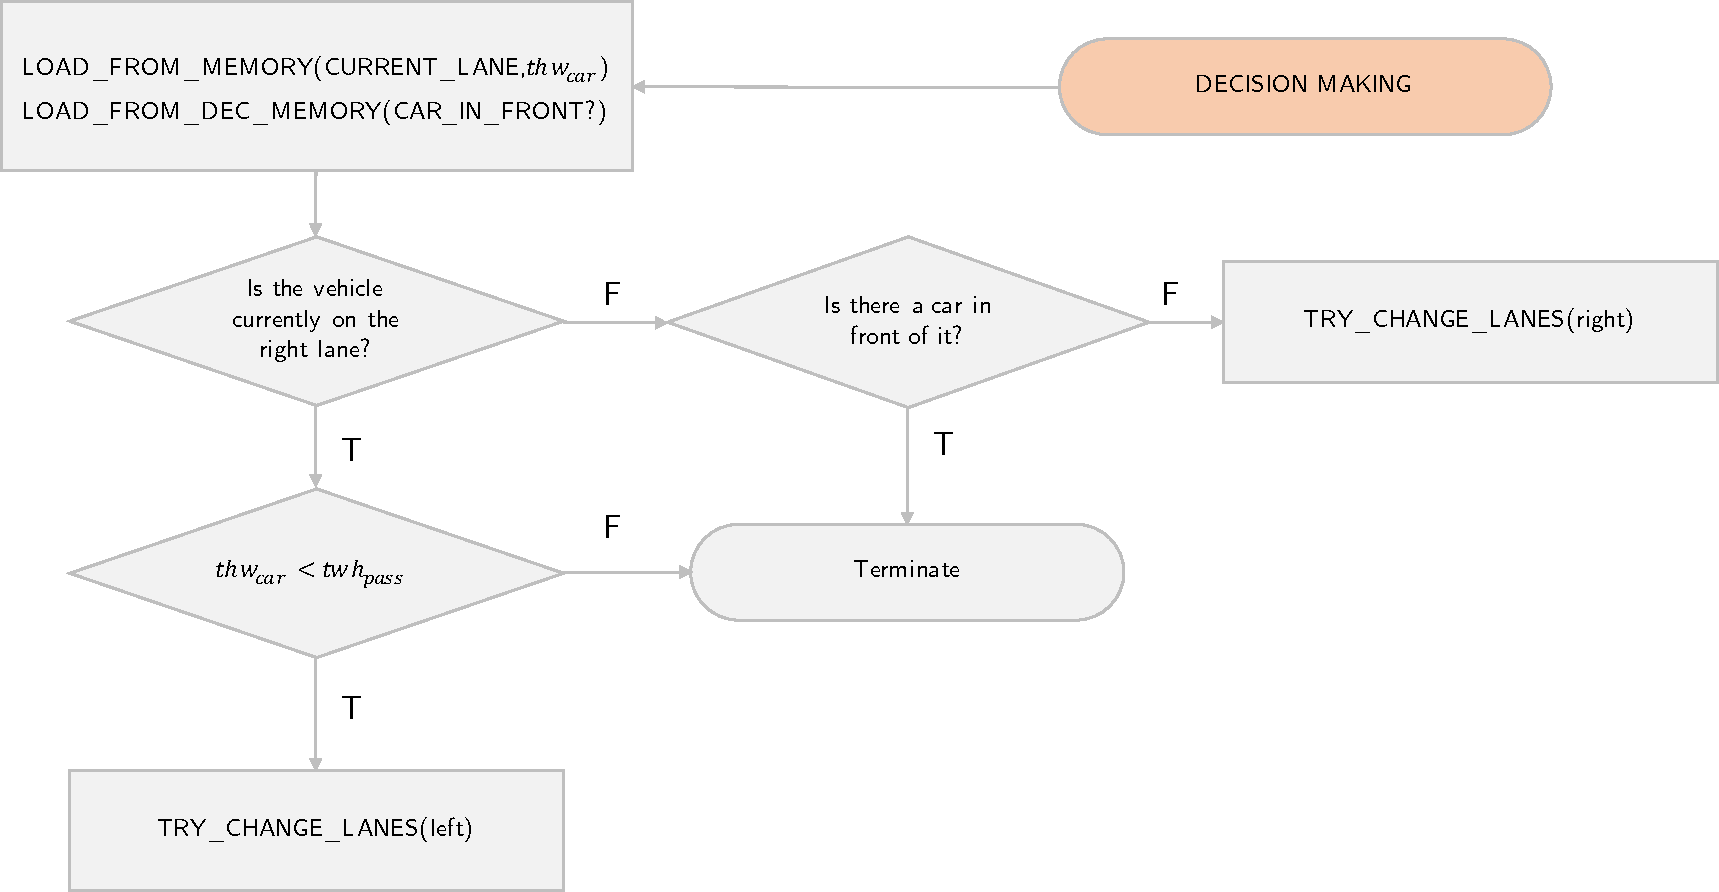
\includegraphics[width=1\textwidth]{dm_1.pdf}
\end{subfigure}\\ \vspace{2em}
\begin{subfigure}{1\textwidth}
  \centering
  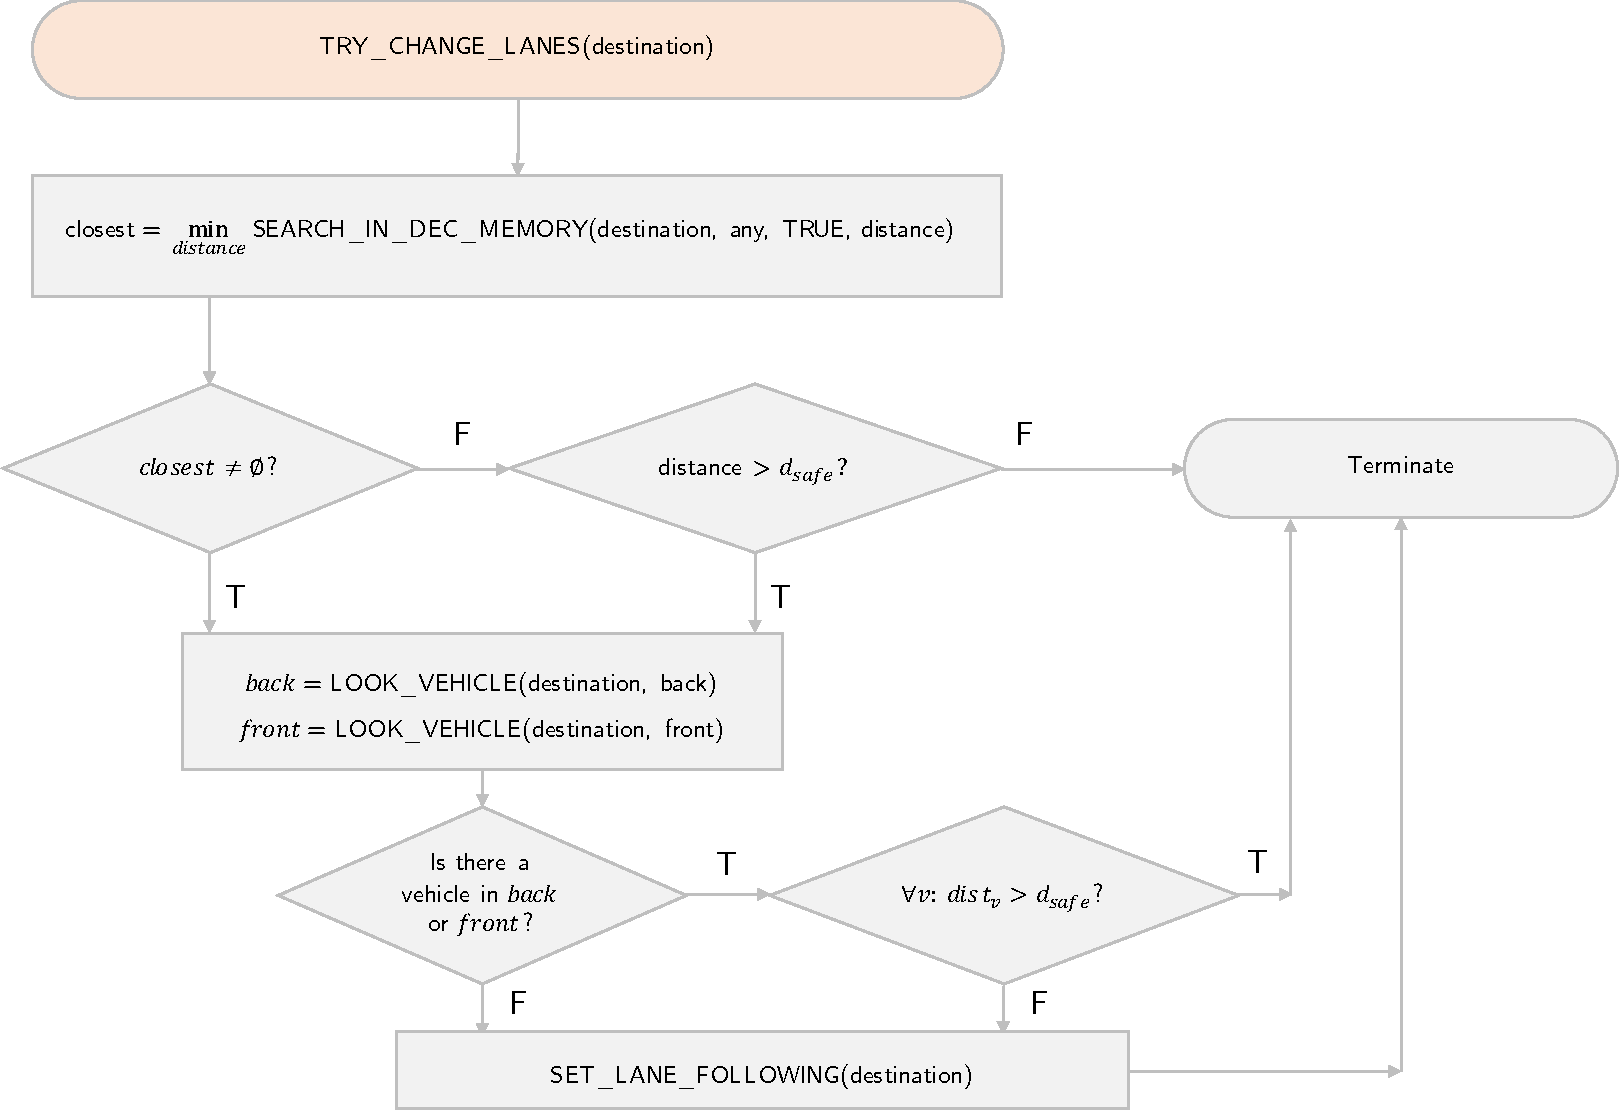
\includegraphics[width=1\linewidth]{dm_2.pdf}
\end{subfigure} \vspace{2em}
\caption{Flowchart of the Decision Making module.}
\label{fig:dm}
\end{figure}

\begin{figure}
\centering
\begin{subfigure}{1\textwidth}
  \centering
  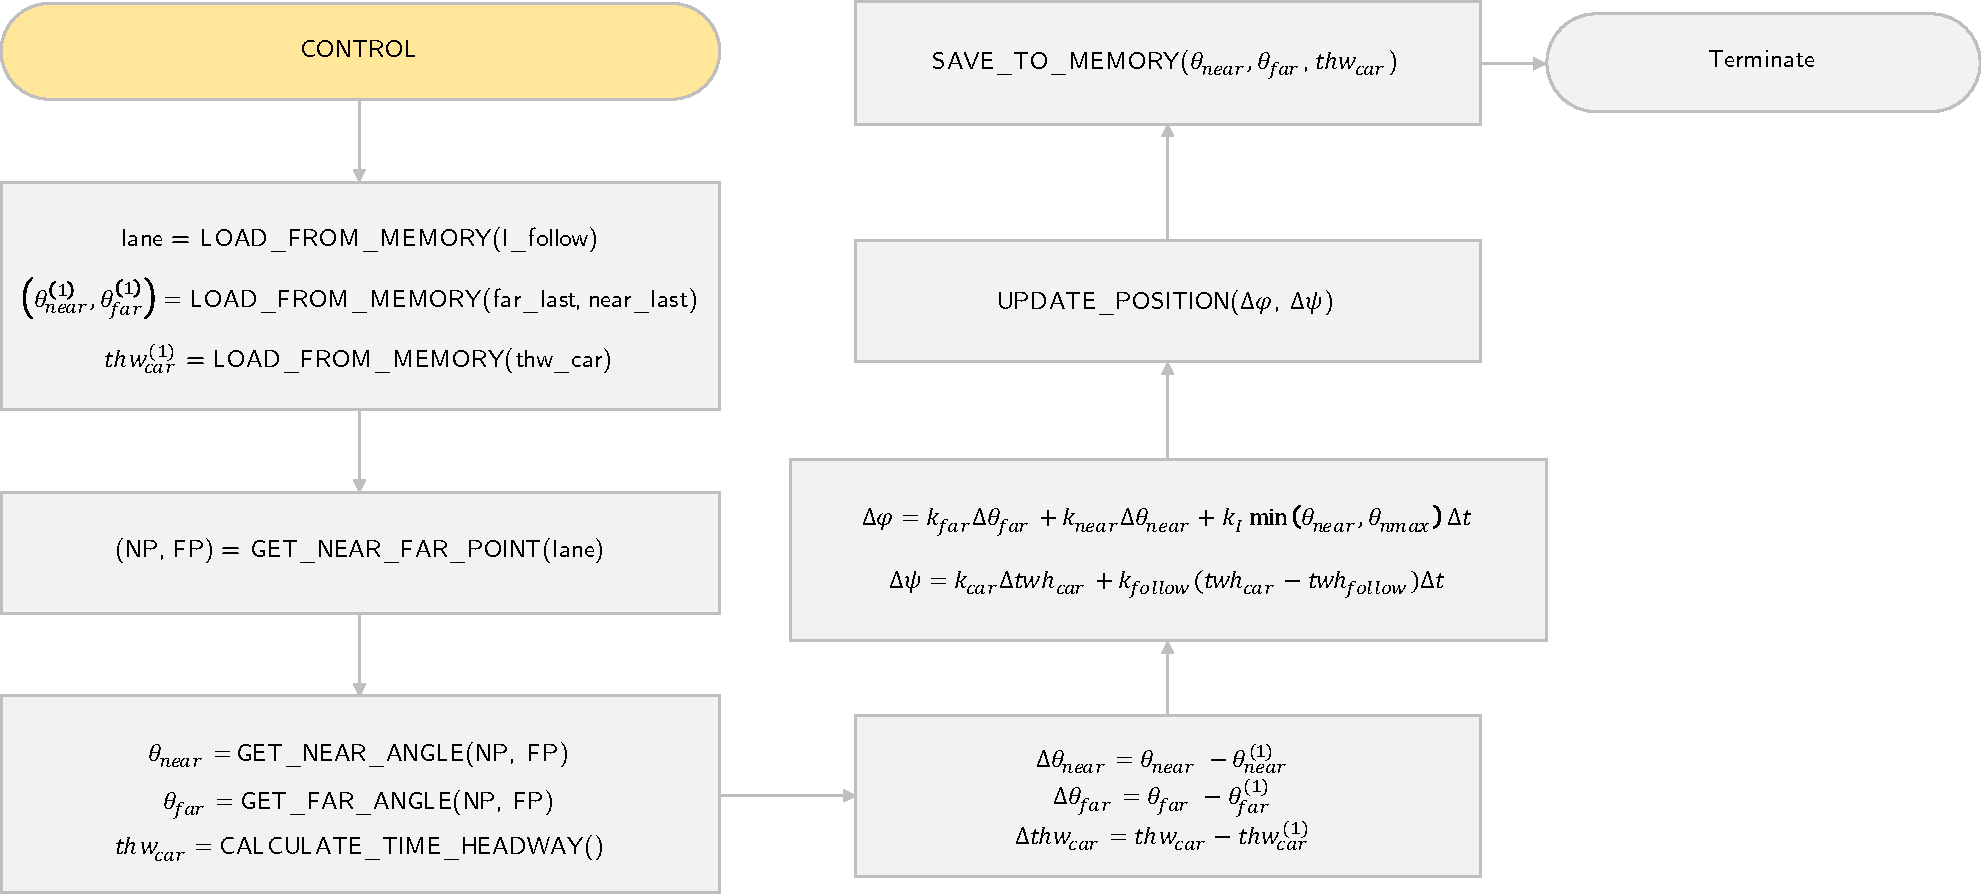
\includegraphics[width=1\textwidth]{control_1.pdf}
\end{subfigure}\\ \vspace{2em}
\begin{subfigure}{1\textwidth}
  \centering
  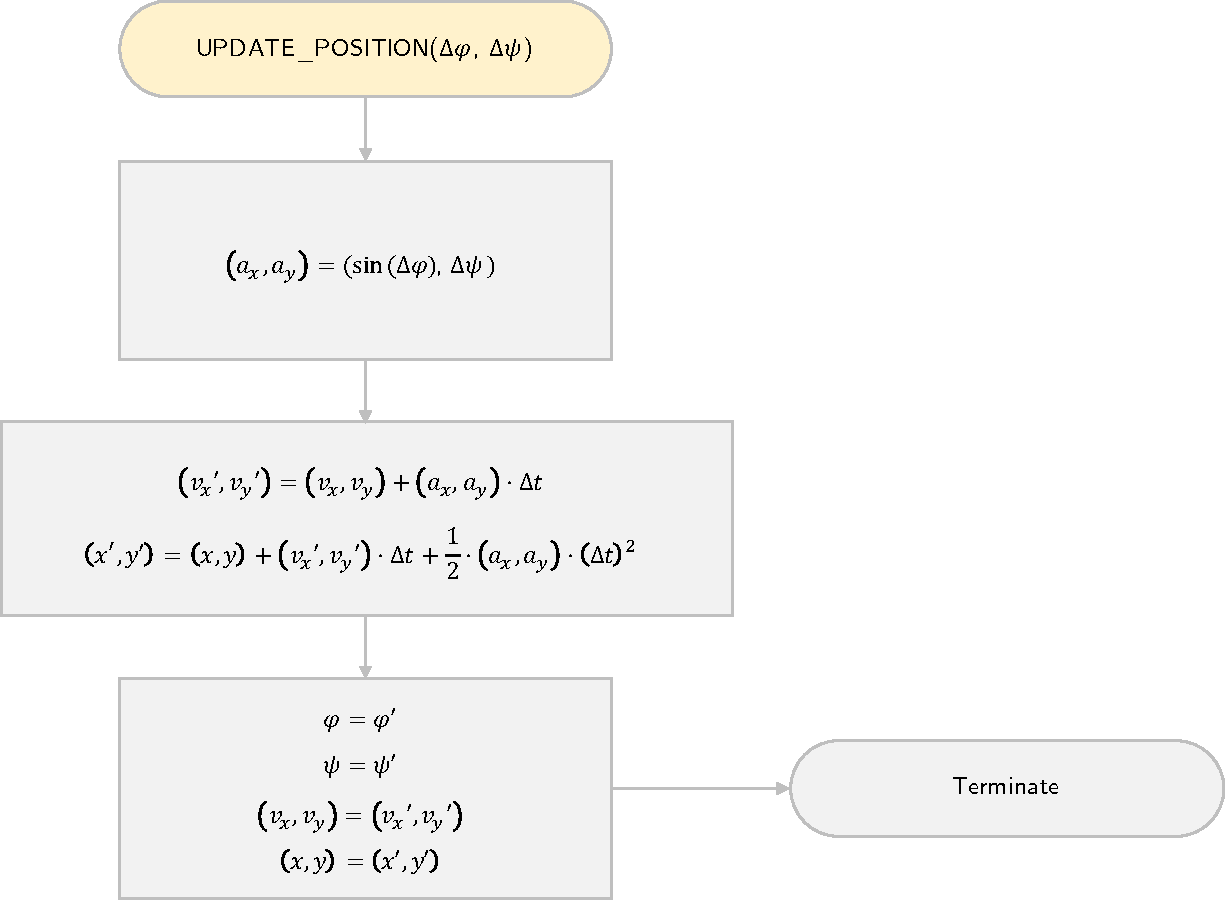
\includegraphics[width=0.7\linewidth]{control_2.pdf}
\end{subfigure} \vspace{2em}
\caption{Flowchart of the Control module.}
\label{fig:control}
\end{figure}

In this case, as Salvucci mentions in \cite{salvucci_1}, $\Delta t = 0.5s$. It is also assumed that the vehicle complies with the speed limits, and, therefore, $v_x \in [15, 34]\text{ }m/s$ (between $50km/h$ and $120km/h$ - typical limits in highway speeds).

Using these assumptions, the continuous driver model is implemented in \textit{Matlab} as presented in Appendix~\ref{sec:appendix_cont}.

\section{Model Abstraction}

The process of abstraction consists in transforming the evolution of the continuous variables that constitute the model and discretising it in order to obtain a finite discrete model. In this case, the goal is to go from the continuous model of driver behaviour presented in the previous section to a discrete-time Markov chain (DTMC) which represents the same process. This transformation is less than trivial due to the fact that, in model checking of finite state abstractions, as the number of state variables in the system increases, the size of the system state space grows exponentially \cite{state_explosion}. This problem is known as state explosion, and there has been some research into efficient ways of dealing with it \cite{abstraction_1, abstraction_2}. 

In the following sections, the abstraction process for the different modules of ACT-R is presented in detail, as well as the thought process behind the choices made. Finally, the unified model is presented using the different modules designed.

\subsection{Non-Probabilistic Control Module}
\label{sec:non_prob_control}

The control module, as presented in the previous section and following Salvucci's approach in \cite{salvucci_1}, is fully deterministic, in the sense that there is no probabilistic reasoning involved. It makes use of perception (for the near and far points) and two simple control laws which influence the position, velocity and acceleration of the vehicle in the environment.

The straightforward approach to this problem would be to represent it as a simple $N\times M$ grid, in which a tuple $(x,y)$ with $x\in \{0,...,N\}$ and $y\in \{0,...,M\}$ would describe the position of the vehicle, and all other variables (i.e. $v_x$, $v_y$, $a_x$, $a_y$ and $t$) would be integer versions of its continuous model representation. In this approach, the control laws could be applied directly over the grid and the results would be the movement of the vehicle in it. However, there is an intrinsic problem with this approach. The error associated with the use of the grid as a way to discretise space would, logically, be reduced with an increase of $N$ and $M$ for a representation of the same road segment (i.e. increase in resolution). For example, the error associated with a road segment of $500 \times 7m^2$ represented by $N = 500$ and $M = 7$ (each grid square corresponds to $1m^2$) would be significantly greater than if $N = 5000$ and $M = 70$ (each grid square corresponds to  $10^{-2}\text{ }m^2$). The conclusion would be that one should increase $N$ and $M$ in order to obtain an appropriate resolution, but this incurs in the problem of state explosion presented in the beginning of the section: as the variable ranges increase, the number of states in the system grows exponentially. Thus, while the situation of $N = 5000$ and $M = 70$ is appealing in terms of error minimisation, it would be intractable to actually build and perform model checking on it (e.g. for $v_x, v_y \in \{15,...,34\}$ and $a_x, a_y \in \{-3,...,3\}$, the control module alone would have approximately $6.89\times 10^{9}$ states, making it impossible to add decision making and monitoring on top of it). 

The straightforward strategy is not, by any standards, efficient in terms of state space and does not use any of the information of the problem to simplify it. In particular, one should notice that, in this scenario, the movement in the $y$ direction is used simply for the purpose of lane changing, a process which is purely deterministic (as described in \cite{salvucci_1}). Therefore, a more interesting approach to the abstraction of the control module could take this into account and \textbf{pre-simulate the lane changing operations}.

In this approach, the vehicle's position is represented by two discrete integer variables $x \in \{0,...,length\}$ for a given $length$ and $lane \in \{right, left\}$ (can be extended to more than two lanes), and the acceleration and velocity of the vehicle are simply $a = a_x$ and $v = v_x$. Time is still represented in the same way, with $t \in \{0,...,max\_time\}$. If a lane change is decided by the decision making module, then, \textbf{within one transition of the control}, the $lane$ variable is updated with the final destination lane, and the variables $x, v, a$ and $t$ are updated to reflect the obtained values after a lane change. These values are obtained from a look-up table and depend on the distance to the other vehicle ($d$) and the velocities of both the vehicle in question ($v$) and the other vehicle ($v_1$) (an obstacle on the road can be modelled by setting $v_1 = 0$). Additionally, the variable $crashed$ is used to represent whether the vehicle has collided in the process or not. The linear acceleration is implemented similarly using pre-simulation to determine the value of acceleration and the motion law is updated in the model itself.

The continuous model of driver behaviour obtained in the previous section in \textit{Matlab} is used as the basis for the simulation of lane changes and linear acceleration. From this model, look-up tables are obtained which, given an origin lane ($o_{lane}$), a distance to the other vehicle and the velocities of both the vehicle in question and the other vehicle determines whether a crash happened or not, what is the $\Delta x$ and $\Delta T$ incurred (how did the position in $x$ changed and how long did it take), and the final velocity of the vehicle in question. The code presented in Appendix~\ref{sec:control_abs} corresponds to a similar version of the control (but probabilistic, as presented later in this section). An example of the simulation of the scenario $o_{lane} = 1$, $d = 20m$, $v = 15m/s$ and $v_1 = 15m/s$ is shown in Figure~\ref{fig:lane_change_ex}.

\begin{figure}[h]
    \centering
    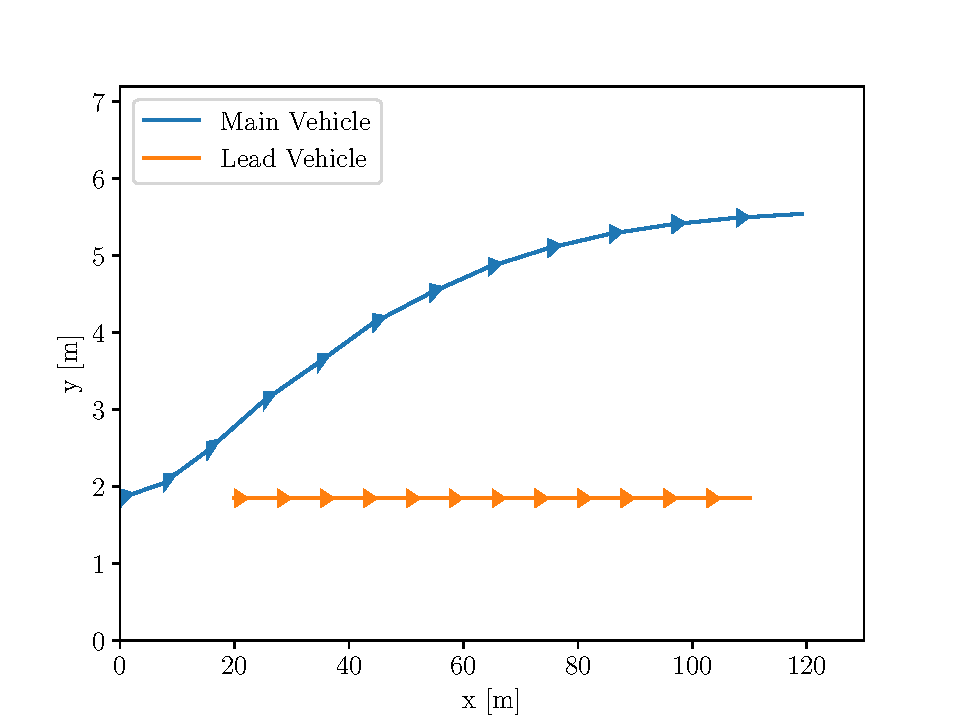
\includegraphics[width=0.9\textwidth]{lane_change_ex.pdf}
    \caption{Example of the simulation of the lane change for $o_{lane} = 1$ (right lane), $d = 20m$, $v = 15m/s$ and $v_1 = 15m/s$. In this case, after the change is complete the variable assignments are $crashed = 0$ (no collision happened), $\Delta x = 119m$, $\Delta T = 6s$ and $v = 23m/s$.}
    \label{fig:lane_change_ex}
\end{figure}

This process focuses the computational effort on the pre-calculations, simplifying the final model significantly in terms of the state space, while removing the error made by discretising in the $y$ direction of the grid (the error in the $x$ direction is still present though). With regards to the size of the lane changing table, for the considered scenario of $2$ lanes, $v, v_1 \in \{15,...,34\}$ and for any discrete $d \in \{1,...,length\}$, the size of the table would be $2\times 20^2 \times length = 800 \times length$. Given that the only value of the table that is effectively altered with a change in $d$ is the value of $crashed$ (as the $\Delta x$, $\Delta T$ and final $v$ depend solely on the initial velocities of both vehicles), it is possible to define $d_{\max}$ such that:

\begin{equation}
d_{\max} < length\text{, s.t. }\forall v, v_1 \in \{15,...,34\}, d' \geq d_{\max}: crashed_{d'} = false
\end{equation}

that is, $d_{\max}$ is a great enough value of $d$ such that, regardless of the speed of the two vehicles, no crash will occur between them. With this change, it is possible to reduce the table from $800\times length$ to $800\times d_{\max}$ (since all other rows would be equal to the one for $d_{max}$). For the given ranges of $v$ and $v_1$, $d_{\max}$ is determined to be $43m$, and thus the obtained look-up table contains $34,400$ rows.

The linear acceleration table depends on the $thw_{car}$ which varies only with the distance to the other vehicle and the current velocity of the vehicle in question. Considering the distance in this case to be up to $80m$ (otherwise maximum acceleration will be applied), the look-up table generated has $1,600$ rows.

\subsection{Decision Making and Monitoring Module}

Due to the fact that, in the model presented by Salvucci in \cite{salvucci_1}, the monitoring module influences the declarative memory which is then used exclusively for decision making purposes (and not for control), logically these two can be incorporated into one for abstraction purposes. Again, taking the straightforward approach of trying to include the declarative memory and the process associated with monitoring and decision making into the model directly would make it intractable. 

In its simplest form, the decision making process for the right lane consists in localising the other vehicle and deciding whether or not to change lanes based on the time headway, $thw_{car}$, to the lead vehicle (if there is one). This value essentially corresponds to the time the vehicle in question has before it crashes into the lead vehicle, assuming that latter came to a full stop ($v = a = 0$) \cite{thw}. The lower this time headway, the more likely a driver is to perform the manoeuvre. While Salvucci presents a fully deterministic driver in \cite{salvucci_1} based on the average driver, in this dissertation it was decided to try and analyse drivers according to different profiles in order to simulate how different parts of the population of drivers might make decisions. The decision making in such a case follows from a stochastic reasoning which can be simulated and incorporated in the model using look-up tables. 

In this case, for a driver in the right lane, it was decided to model the probability of the driver performing a lane change based on the time headway as an exponentially decreasing function, writing it as:

\begin{equation}
	\text{P[}lC = true\text{]}_{thw} = P_{lC}(d,v) = e^{-\alpha\cdot thw} = e^{-\alpha\cdot d/v}
\end{equation}

where $\alpha$ is a parameter unique to each population of drivers. 

The same logic can be applied for a driver in the left lane overtaking a vehicle behind it in the left lane, except in this case the opposite effect will be seen in the decision making. In such a case, the probability of changing lane can be modelled as a normalised logarithmic function over the distance of the vehicles (it doesn't make sense to define time headway in this context):

\begin{equation}
	\text{P[}lC = true\text{]}_{d} = P_{lC}(d) = \frac{1}{\log(\beta*\max_d + 1)}\cdot \log(\beta*d + 1)
\end{equation}

where $\max_d$ is the maximum length considered and $\beta$ is a parameter unique to each population of drivers.

It should be noted that these functions, while logical, are an assumption of the abstraction, since the model presented by Salvucci in \cite{salvucci_1} does not make any reference to these parameterisations. It is also worth referring that, while there was no real-world data involved in this project, this function could have been learnt from real data without changing the fundamental paradigm of the abstraction.

For the purposes of analysis, three classes of drivers are considered: \textbf{Aggressive}, \textbf{Average} and \textbf{Cautious} drivers (with different values for the parameter $\alpha$ and $\beta$). In Figure~\ref{fig:dm_curves}, the functions are presented for the three profiles of drivers assumed in this project, for the lane changes originating in the right (Figure~\ref{fig:dm_curve_right}) and left lane (Figure~\ref{fig:dm_curve_left}).

\begin{figure}
\centering
\begin{subfigure}{1\textwidth}
	\centering
	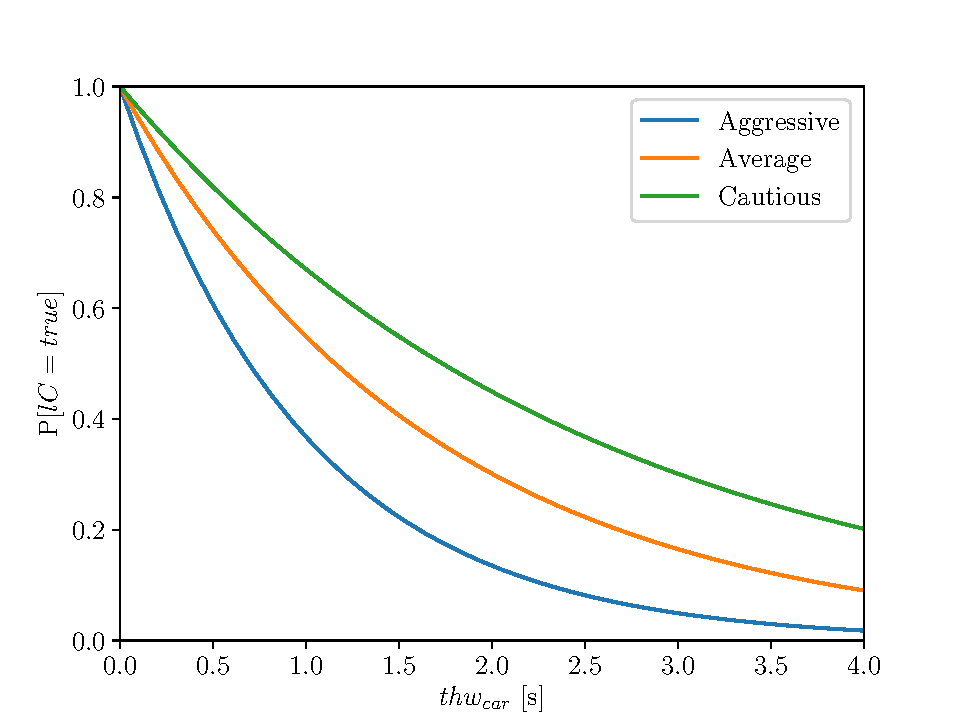
\includegraphics[width=0.85\textwidth]{dm_curve.pdf}
	\subcaption{Aggressive ($\alpha = 1$), Average ($\alpha = 0.6$) and Cautious ($\alpha = 0.4$) drivers.}
	\label{fig:dm_curve_right}
\end{subfigure}\\
\begin{subfigure}{1\textwidth}
	\centering
	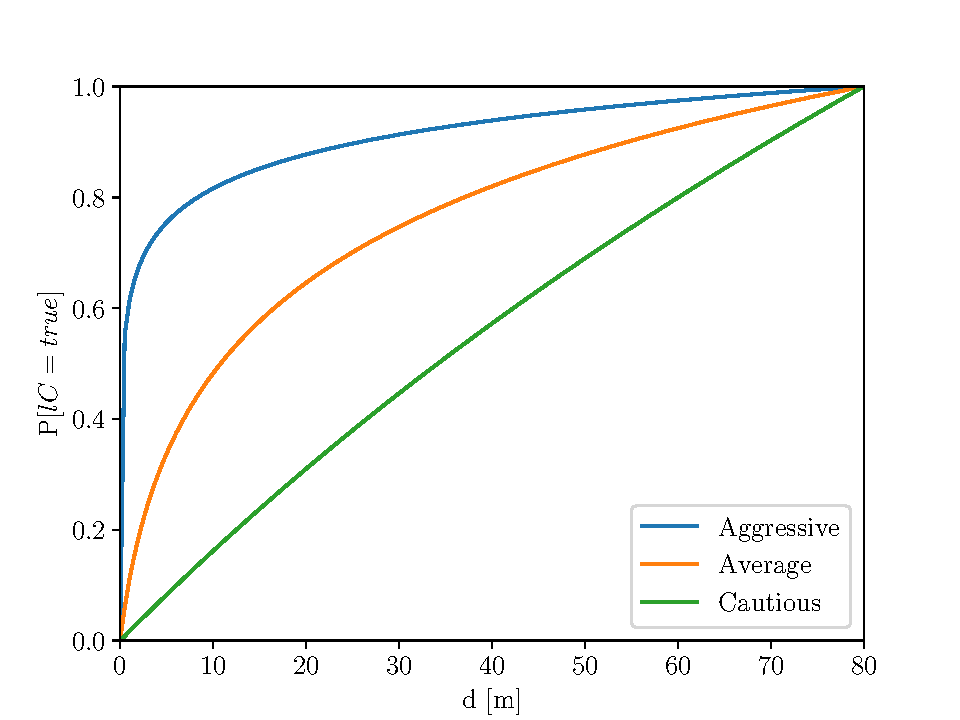
\includegraphics[width=0.85\textwidth]{dm_curve_2.pdf}
	\subcaption{Aggressive ($\beta = 1000$), Average ($\beta = 0.5$) and Cautious ($\beta = 0.01$) drivers.}
	\label{fig:dm_curve_left}
\end{subfigure}\vspace{1em}
\caption{$\text{P[}lC = true\text{]}$ as a function of $thw_{car}$ and $d$ for vehicles originating from the right lane (a) and left lane (b).}
\label{fig:dm_curves}
\end{figure}

So far, this version of decision making is not influenced by the monitoring module at all, and it relies on the correct calculation of the value of $thw_{car}$ and $d$. This assumption is unrealistic, and in order to simulate these issues, it was decided that stochastic noise could be added to the measurement of the distance (as this is what human drivers have to instinctively measure through perception). It was chosen that this noise, $n$, would be normally distributed as:

\begin{equation}
	n \sim \mathcal{N}(0, \sigma)
\end{equation}

such that:

\begin{equation}
	thw'_{car} = thw_{car} + n(thw_{car})
\end{equation}

Alternatively, this can be represented directly as (using discrete integration steps of width $\delta$):

\begin{equation}
\begin{aligned}
	P'_{lC}(d,v) & = \sum_{i = -\infty}^{+\infty} [N(d + i + \delta/2) - N(d + i - \delta/2)] \cdot P_{lC}(d + i,v) \\
	& = \sum_{i = -\max_d}^{+\max_d} [N(d + i + \delta/2) - N(d + i - \delta/2)] \cdot P_{lC}(d + i,v)
\end{aligned}
\end{equation}

where $\max_d$ is the maximum length considered and $N(d)$ corresponds to the cumulative probability function (CDF) defined as:

\begin{equation}
	N(d) = \int_{-\infty}^d n(t) dt
\end{equation}

From this, a look-up table can be generated which, for different driver types, yields the probability of lane changing for a certain distance to the lead car and velocity. For the 3 driver profiles mentioned, considering $d \in \{1,...,80\}$ ($\max_d = 80$) and $v \in \{15,...,34\}$, the table generated for the vehicle in the right lane has $4,800$ rows \footnote{In the data obtained for the results presented in this dissertation, $\delta = 1$.}. Under the same conditions, the look-up table for the vehicle in the left obtained has $240$ rows (the difference is explained by the fact that the velocity does not influence this table). Thus, the unified decision making table has $5,040$ rows.

The code presented in Appendix~\ref{sec:dm_abs} corresponds to the methods used to obtain the unified look-up table used for the decision making and monitoring module.

\subsection{Probabilistic Control Module}
\label{sec:prob_control}

In light of the uncertainty introduced in the decision making and monitoring module regarding the visual perception of distance, it becomes only natural that this would be extended to the control module as well. In order to cope with this, a probabilistic version of the control module was designed, where the noise $n$ presented in the previous section is taken into consideration. 

In order to obtain the equivalent look-up tables for the probabilisitic control module, the Monte Carlo method can be used. In this case, the noise can be simulated in repeated trials, and an average can be obtained for the crashing probability, the estimated final difference in position, the estimated difference in time and estimated final velocity of the vehicle. In the case of this dissertation, the tables generated (for linear and lane changing control) were the result of 100 trials.

The code presented in Appendix~\ref{sec:control_abs} corresponds to the simulation of this probabilistic version of the control, which generates the linear and steering control tables.

\subsection{Unified Two-Module Model}

Using the three tables generated (two for the probabilisitic control - linear and steering control - and one for the decision making), the final DTMC model unifies both using a sequential variable $actr\_state \in \{1,2\}$, where $actr\_state = 1$ corresponds to the control and $actr\_state = 2$ corresponds to decision making. In the version of the unified model built for this thesis, only two vehicles are present: the first is the one controlled by the driver and the second is a lead vehicle starting at a distance $x = x_{1,0}$ (in meters) from the main vehicle (which starts at $x=0$) and moves with a constant speed of $v_1$ on a road segment of $length$ meters. The movement of the lead vehicle is, therefore, completely determined by the formula:

\begin{equation}
	x_1(t) = x_{1,0} + v_1\cdot t
\end{equation}

The distance between the two vehicles can be obtained as:

\begin{equation}
	d(t) = \lvert x(t) - x_1(t) \rvert
\end{equation}

And the boolean function $posDist$ can be defined as:

\begin{equation}
posDist(t) = 
     \begin{cases}
       \text{true,} &\quad\text{if }x(t) \geq x_1(t)\\
       \text{false,} &\quad\text{otherwise.} \\
     \end{cases}
\end{equation}

Due to the large size of the tables generated, the models should be generated automatically for a given tuple of initial conditions $(d_{type}, v, v_1, x_{1,0})$ (where $d_{type}$ is the driver class according to the ones defined in the decision making and monitoring subsection - 1 is aggressive, 2 is average and 3 is cautious), following the assumptions described below:

\textbf{General assumptions}

\begin{enumerate}
	\item A transition from state $s$ to state $s'$ is possible if, and only if, the variable $actr\_state$ takes different values in $s$ and $s'$.
	\item A transition from state $s$ to state $s'$ is possible if, and only if, $t_{s'} \geq t_s$ (where $t_{\alpha}$ is the value of variable $t$ in state $\alpha$).
	\item The model should have no states with self transitions, as there is always a continuous evolution of the state of the vehicles.
	\item A deadlock state should only be entered if, and only if, the vehicle either crashes ($crashed = true$) or reaches the end of the road ($x = length$).
\end{enumerate}

\textbf{Control ($actr\_state = 1$)}

\begin{enumerate}
	\item If no lane change has been decided, the model reasons over linear acceleration using the corresponding look-up table for $d(t)$ and $v(t)$, and updates the state variables $t, x, v, a$ and $crashed$ accordingly using the discrete laws of motion previously presented.
	\item If a lane change has been decided, the model reasons over the lane change using the corresponding look-up table for $o_{lane}$, $d(t)$, $v(t)$, $v_1$, and updates the variables $x$ and $t$ incrementally using the values $\Delta x$ and $\Delta T$ of the table, as well as sets the value of $v$ and $crashed$.
\end{enumerate}

\textbf{Decision Making and Monitoring ($actr\_state = 2$)}

\begin{enumerate}
	\item If the vehicle is on the left lane and behind the other vehicle ($lane=left$ and $posDist = false$), the model will not attempt a lane change.
	\item If the vehicle is on the left lane and in front of the other vehicle ($lane=left$ and $posDist = true$), the model will reason over lane changes using the decision making and monitoring look-up table for $d_{type}$.
	\item If the vehicle is on the right lane and behind the other vehicle ($lane=right$ and $posDist = false$), the model will reason over lane changes using the decision making and monitoring look-up table for $d_{type}$.
	\item If the vehicle is on the right lane and in front of the other vehicle ($lane=left$ and $posDist = true$), the model will not attempt a lane change.
\end{enumerate}

From these rules and the tables obtained in the abstraction of the individual modules, it is possible to build a model generator. The code for an example of such a generator written in \textit{Python} (used throughout the rest of the dissertation) is presented in Appendix~\ref{sec:two_module_gen}. 

By running the model generator using the conditions $(d_{type}, v, v_1, x_{1,0}) = (1,30,22,51)$, that is, an aggressive driver, starting at $30m/s$ with another vehicle going at $22m/s$ and starting at $51m$, the resulting model description is the one presented in Listing~\ref{lst:model_example} (shortened for the sake of space saving; the full model is $13,435$ lines long).

{\vspace{1em}
\begin{lstlisting}[caption={Example of the model generated for the tuple $(d_{type}, v, v_1, x_{1,0}) = (1,30,22,51)$ (shortened)},captionpos=b,label={lst:model_example}]
//Model automatically built using model_generator.py for v1 = 22 and driver_type = 1 (to alter these values, run the script again).
//Generated on 31-07-2018 at 18:47.

dtmc

const int length = 500; // road length
const int driver_type = 1; // 1 = aggressive, 2 = average, 3 = cautious drivers - do not alter this manually!
const int max_time = 35; // maximum time of experiment

// Other vehicle
const int v1 = 22; // do not alter this manually!
const int x1_0 = 51;

// Environment variables
global t : [0..max_time] init 0; // time 
global crashed : bool init false; 

// Vehicle controlled
global actrState : [1..2] init 1; // active module: 1 = control (both cars), 2 = decision making + monitoring
global lC : bool init false; // lane changing occuring? 
global x : [0..length] init 0;
global v : [15..34] init 30;
global a : [-2..3] init 0;
global lane : [1..2] init 1;

formula x1 = x1_0 + v1*t;
formula dist = x1>x?(x1 - x):(x - x1);
formula positiveDist = (x < length)?x > x1:true;

module Decision_Making_Monitoring

 	// If a crash occurs, then nothing else can happen
	//[] actrState = 2 & crashed -> 1:(crashed' = true);

 	// If we are in lane 2, but behind the other vehicle, don't try to pass
	[] actrState = 2 & !crashed & lane = 2 & positiveDist = false -> 1:(actrState' = 1);

	// If we are in lane 1, and no vehicle is in front, don't change lanes
	[] actrState = 2 & !crashed & lane = 1 & positiveDist = true -> 1:(actrState' = 1);

	[] actrState = 2 & !crashed & lane = 1 & positiveDist = false & dist = 1 & v = 15 -> 0.8:(actrState' = 1) & (lC' = true) + 0.2:(actrState' = 1) & (lC' = false);

	...

	[] actrState = 2 & !crashed & lane = 2 & positiveDist = true & dist >= 80 -> 1:(actrState' = 1) & (lC' = true) + 0:(actrState' = 1) & (lC' = false);
endmodule

module Control

 	// If we are in lane 1, and no lane change was decided, continue forward (which might result in crash)
 	// The vehicle is behind the other driver (positiveDist = false, x < x1)
	[] actrState = 1 & !crashed & !lC & lane = 1 & x <= length - v & t < max_time & positiveDist = false & (x1 + v1 - x - v) >= 6 & v + a < 34 & v + a > 15 & dist = 1 & v = 15  -> 1:(x' = x + v) & (t' = t + 1) & (v' = v + a) & (a' = -2) & (actrState' = 2);

	...

	[] actrState = 1 & !crashed & lC & lane = 2 & dist >= 43 & v = 34 & x > length - 136 & t > max_time - 6 -> 1:(crashed' = false) & (x' = length) & (v' = 34) & (t' = max_time) & (a' = 0) & (lane' = 1) & (actrState' = 2) & (lC' = false);

endmodule
\end{lstlisting}
}

By loading and building the model in either PRISM or Storm, it is observable that it has 257 states and 295 transitions, a significant reduction from the possibilities presented in the straightforward control abstraction. Due to the fact that there are $3\times 20 \times 20 \times length$ different possibilities in terms of initial conditions, it would be intractable, in the timeline of the dissertation, to obtain the number of states for all the combinations. Table~\ref{tab:sta_tra_example} presents the number of states and transitions for some arbitrarily generated conditions (for a road of length $500m$).

{
\vspace{1em}
\bgroup
\def\arraystretch{1.3}
\begin{table}[h]
\centering
\begin{tabular}{|c|c|c|c||c|c|}
\hline
\textbf{$d_{type}$} & \textbf{$v$} & \textbf{$v_1$} & \textbf{$x_{1,0}$} & \textbf{\# States} & \textbf{\# Transitions} \\ \hline \hline
3 & 21 & 30 & 20 & 305 & 333 \\ \hline
1 & 27 & 22 & 66 & 396 & 471 \\ \hline
1 & 28 & 17 & 43 & 167 & 183 \\ \hline
2 & 33 & 15 & 35 & 6 & 7 \\ \hline
3 & 28 & 21 & 38 & 199 & 222 \\ \hline
1 & 19 & 16 & 81 & 391 & 443 \\ \hline
2 & 25 & 23 & 28 & 390 & 481 \\ \hline
3 & 15 & 17 & 36 & 487 & 569 \\ \hline
1 & 29 & 18 & 74 & 201 & 220 \\ \hline
2 & 31 & 29 & 52 & 234 & 265 \\ \hline
\end{tabular}
\caption{Results of the number of states and transitions for arbitrary initial conditions.}
\label{tab:sta_tra_example}
\end{table}
\egroup
}

\section{Model Evaluation Metrics}
\label{sec:model_metrics}

With the model efficiently represented as a DTMC through abstraction, it becomes possible to perform model checking of certain properties on it in order to evaluate the relative performance of different profiles of drivers. In the following subsections, different categories of evaluation are presented and properties representing metrics within that category are proposed and tested in a small population of scenarios (the same test cases used to generate  Table~\ref{tab:sta_tra_example}). In the rest of the dissertation it is assumed (unless explicitly mentioned otherwise) that the road segment has a length of $500m$.

\subsection{Completeness Properties}

From the rules used to build the model, it is explicit that a correct model should only enter a deadlock if it crashes or the vehicle reaches the end of road. As such, it is expected that every path from the initial state leads to states where the vehicle is in one of those two conditions. This property can be explicitly written as:

\begin{minipage}{\linewidth}
{\vspace{1em}
\begin{lstlisting}
P>=1 [F (crashed | x=length)]
\end{lstlisting}
}
\end{minipage}

and it tests whether a model is complete by verifying that every possible outcome satisfies the restrictions imposed (regardless of the value of the other variables). Additionally, both PRISM and Storm allow the following property to be verified:

\begin{minipage}{\linewidth}
{\vspace{1em}
\begin{lstlisting}
P>=1 [F "deadlock"]
\end{lstlisting}
}
\end{minipage}

which guarantees that a deadlock will eventually be reached and no infinite loop  is generated by mistake within the DTMC.

Using PRISM or Storm, the results of the model checking of these properties in the test cases are presented in Table~\ref{tab:completeness}. As expected, for all the scenarios the properties are satisfied, confirming that these models are complete in terms of the expected outcome. While these properties do not need to be extensively analysed, they constitute a guarantee that the generated model is complete. As such, its verification is performed in all tests done in the analysis of Chapter~\ref{sec:results}.

{
\vspace{1em}
\bgroup
\def\arraystretch{1.3}
\begin{table}[h]
\centering
\begin{tabular}{|c|c|c|c||c|c|}
\hline
\textbf{$d_{type}$} & \textbf{$v$} & \textbf{$v_1$} & \textbf{$x_{1,0}$} & \texttt{P>=1 [F (crashed | x=length)]} & \texttt{P>=1 [F "deadlock"]} \\ \hline \hline
3 & 21 & 30 & 20 & \texttt{true} & \texttt{true} \\ \hline
1 & 27 & 22 & 66 & \texttt{true} & \texttt{true} \\ \hline
1 & 28 & 17 & 43 & \texttt{true} & \texttt{true} \\ \hline
2 & 33 & 15 & 35 & \texttt{true} & \texttt{true} \\ \hline
3 & 28 & 21 & 38 & \texttt{true} & \texttt{true} \\ \hline
1 & 19 & 16 & 81 & \texttt{true} & \texttt{true} \\ \hline
2 & 25 & 23 & 28 & \texttt{true} & \texttt{true} \\ \hline
3 & 15 & 17 & 36 & \texttt{true} & \texttt{true} \\ \hline
1 & 29 & 18 & 74 & \texttt{true} & \texttt{true} \\ \hline
2 & 31 & 29 & 52 & \texttt{true} & \texttt{true} \\ \hline
\end{tabular}
\caption{Results of the verification of the completeness properties.}
\label{tab:completeness}
\end{table}
\egroup
}

\subsection{Safety Property}

One essential evaluation metric of the human driver is its capability of driving safely, i.e. without crashing. To that effect, the following safety property is devised:

\begin{minipage}{\linewidth}
{\vspace{1em}
\begin{lstlisting}
P=? [F crashed]
\end{lstlisting}
}
\end{minipage}

It should be noted that, for a given set of initial conditions, the lower the quantitative value of the property, the safer the driver is. From the assumptions made in the abstraction process, it is expected that Aggressive drivers will perform worse than Average ones in this metric, which in turn will perform worse than Cautious drivers. Extensive experimental results regarding this property are presented in Chapter~\ref{sec:results}. The results of the verification of the safety property in the test cases are presented in Table~\ref{tab:safety}. It can observed that these vary quite significantly according to the situation, with the quantitative values ranging from $0.0193$ (unlikely to crash) to $1$ (will crash with certainty).

{
\vspace{1em}
\bgroup
\def\arraystretch{1.3}
\begin{table}[h]
\centering
\begin{tabular}{|c|c|c|c||c|c|}
\hline
\textbf{$d_{type}$} & \textbf{$v$} & \textbf{$v_1$} & \textbf{$x_{1,0}$} & \texttt{P=? [F crashed]} \\ \hline \hline
3 & 21 & 30 & 20 & 0.0232 \\ \hline
1 & 27 & 22 & 66 & 0.3017 \\ \hline
1 & 28 & 17 & 43 & 0.7119 \\ \hline
2 & 33 & 15 & 35 & 1 \\ \hline
3 & 28 & 21 & 38 & 0.1604 \\ \hline
1 & 19 & 16 & 81 & 0.6074 \\ \hline
2 & 25 & 23 & 28 & 0.0562 \\ \hline
3 & 15 & 17 & 36 & 0.0276 \\ \hline
1 & 29 & 18 & 74 & 0.5123 \\ \hline
2 & 31 & 29 & 52 & 0.0193 \\ \hline
\end{tabular}
\caption{Results of the verification of the safety property.}
\label{tab:safety}
\end{table}
\egroup
}

\subsection{Liveness Properties}
\label{sec:live_props}

Liveness can be defined in terms of the efficiency of the drivers, i.e. how quickly do they reach the end of the road. One of the variables of the model is the time, $t$, in seconds since the beginning of the execution. For a given constant $T$, the property:

\begin{minipage}{\linewidth}
{\vspace{1em}
\begin{lstlisting}
P=? [F (x=length & t < T)]
\end{lstlisting}
}
\end{minipage}

captures the probability of reaching the end within less than $T$ seconds. It should be noted that this constant $T$ needs to be adjusted to different values in order to test specific properties, so this property should actually be defined as the list of properties:

\begin{minipage}{\linewidth}
{\vspace{1em}
\begin{lstlisting}
P=? [F (x=length & t < 1)]
P=? [F (x=length & t < 2)]
...
P=? [F (x=length & t < max_time-1)]
P=? [F (x=length & t < max_time)]
\end{lstlisting}
}
\end{minipage}

However, the problem with these properties is based on the fact that they intrinsically rely on the safety property, since a higher probability of crashing naturally implies a lower probability of reaching the end, and, therefore, an even lower probability of reaching the end under $T$ seconds. To mitigate this issue, the following conditional properties are introduced:

\begin{minipage}{\linewidth}
{\vspace{1em}
\begin{lstlisting}
P=? [F (x=length & t<T) || F (x=length)]
\end{lstlisting}
}
\end{minipage}

which reads as \textit{"what is the probability that the model eventually reaches a state where }\texttt{x = length}\textit{ and }\texttt{t < T}\textit{ given that it reaches one where} \texttt{x = length}\textit{"}. This allows for direct comparisons between driver profiles and different scenarios. It should be noted that these are actually $max\_time$ different properties, as with the case of the unconditional ones. 

Using Storm, both the unconditional and conditional properties can be verified directly. While PRISM supports the unconditional ones, conditional properties are not yet supported by the tool. However, it is possible to verify separately the properties \texttt{P=? [F (x=length \& t<T)]} and \texttt{P=? [F (x=length)]}, and use Bayes' theorem to calculate:

\begin{equation}
\text{\texttt{P=? [F (x=length \& t<T) || F (x=length)]}} = \frac{\text{\texttt{P=? [F (x=length \& t<T)]}}}{\text{\texttt{P=? [F (x=length)]}}}
\end{equation}

Table~\ref{tab:liveness} presents the results of the verification of the liveness properties in the test cases. In the interest of brevity, only two of each (unconditional and conditional) properties verified are presented, for $T = 19$ and $T = 24$ (arbitrarily selected), and they will be identified using the following number system (for presentation purposes):

\begin{minipage}{\linewidth}
{\vspace{1em}
\begin{lstlisting}
1. P=? [F (x=length & t<19)]
2. P=? [F (x=length & t<24)]
3. P=? [F (x=length & t<19) || F (x=length)]
4. P=? [F (x=length & t<24) || F (x=length)]
\end{lstlisting}
}
\end{minipage}

\bgroup
\def\arraystretch{1.3}
\begin{table}[h]
\centering
\begin{tabular}{|c|c|c|c||c|c||c|c|}
\hline
\textbf{$d_{type}$} & \textbf{$v$} & \textbf{$v_1$} & \textbf{$x_{1,0}$} & \texttt{1} & \texttt{2} & \texttt{3} & \texttt{4}  \\ \hline \hline
3 & 21 & 30 & 20 & 0.0085 & 1 & 0.0085 & 1 \\ \hline
1 & 27 & 22 & 66 & 0.5908 & 0.6983 & 0.8460 & 0.9999 \\ \hline
1 & 28 & 17 & 43 & 0 & 0.2881 & 0 & 1 \\ \hline
2 & 33 & 15 & 35 & 0 & 0 & 0 & 0 \\ \hline
3 & 28 & 21 & 38 & 0 & 0.8396 & 0 & 1 \\ \hline
1 & 19 & 16 & 81 & 0 & 0.3926 & 0 & 0.9999 \\ \hline
2 & 25 & 23 & 28 & 0.1555 & 0.9438 & 0.1648 & 0.9999 \\ \hline
3 & 15 & 17 & 36 & 0 & 0.5849 & 0 & 0.6015 \\ \hline
1 & 29 & 18 & 74 & 0.4662 & 0.4877 & 0.9559 & 1 \\ \hline
2 & 31 & 29 & 52 & 0.9992 & 0.9992 & 1 & 1 \\ \hline
\end{tabular}
\caption{Results of the verification of the liveness properties.}
\label{tab:liveness}
\end{table}
\egroup

From Table~\ref{tab:liveness}, it is possible to observe that different scenarios, despite having distinct values of the unconditional properties, have a similar value of the conditional ones. For example, for $T < 24$, the scenario $(d_{type}, v, v_1, x_{1,0}) = (1, 28, 17, 43)$ has a a significantly lower unconditional probability than the $(d_{type}, v, v_1, x_{1,0}) = (3, 28, 21, 38)$, yet they have exactly the same conditional one. While the unconditional properties can be interpreted in these scenarios as \textit{"the vehicle will reach the end of the road and be under 24s with probability 0.2881"} and \textit{"the vehicle will reach the end of the road and be under 24s with probability 0.8396"},  in both these cases the conditional probability should be interpreted as \textit{"if the vehicle reaches the end of the road, then it will do so before 24s with certainty"}. The conditional property can be understood as an elimination of the safety bias inherent to each scenario, leading to more meaningful inter-situational comparisons. Extensive experimental results regarding these properties are presented in Chapter~\ref{sec:results}

\section{Simulation of Paths in the Model}
\label{sec:simulator}

In order to visualise possible executions of the trajectory and decisions taken in the model, a visual simulator was designed and implemented in \textit{Python}, with the code presented in Appendix~\ref{sec:sim-app}.

The simulator essentially uses the option \texttt{simpath} in the PRISM command line tool which allows it to output a simulated path in the model without having to actually build it. Using this outputted path in the model, the script reads it and plays it back to the user using a GUI built in \textit{pygame} for \textit{Python} \cite{pygame}. 

In order to faithfully represent the lane change operations the driver performs, an additional table is obtained using the steering control abstraction, which corresponds to the interpolation of the $x$ and $y$ positions of the vehicle as a function of time (i.e. $x(t)$ and $y(t)$). Given the complexity of the $y$ movement compared to the $x$ movement, the positions are represented by a $6^{th}$ and $2^{nd}$ degree polynomial, respectively. 

Due to the size of the example, only one test case is presented of a simulation of a path in a model. In Figure~\ref{fig:example_sim}, an example of several frames of the simulation of a path in the scenario $(d_{type}, v, v_1, x_{1,0}) = (3, 28, 21, 38)$ is presented. In this case, the driver initiates a lane change to perform an overtake at the 2s mark and returns to the original lane at the 8s mark, with no crashing occurring. In the simulation, the vehicle took $18.3s$ to reach the end of the road. It should be noted that, as verified by the conditional liveness property, the vehicle took less than $24s$ to reach the end of the road segment. While it would appear the vehicle took less than $19s$ to reach the end (and thus would violate the probability of $0$ obtained for this liveness property), the model considers steps of $1s$, so in the model, the vehicle actually took $19s$ to finish instead of $18.3s$.

\begin{figure}[h]
\centering
\begin{subfigure}{0.75\textwidth}
  \centering
  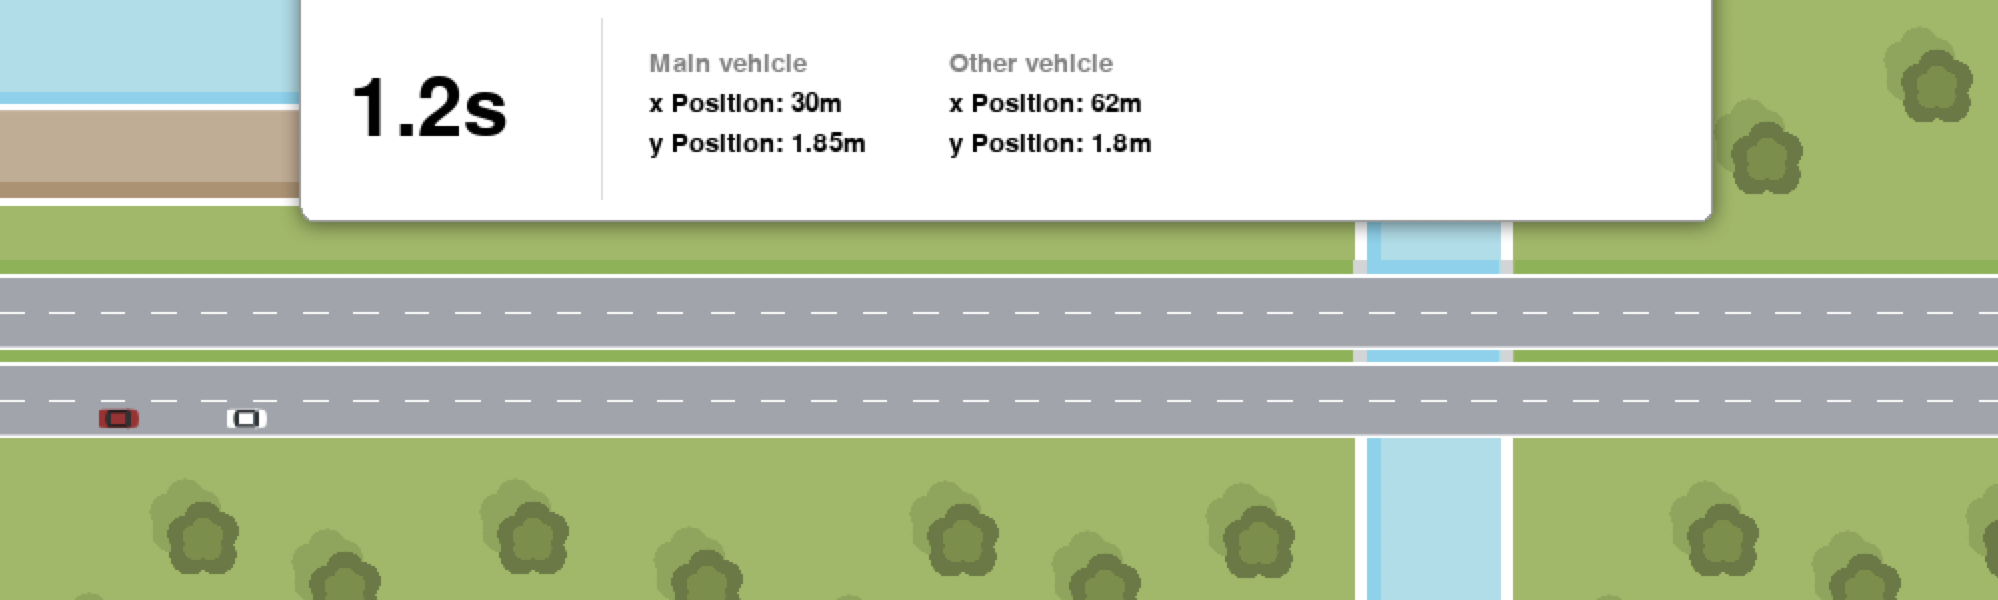
\includegraphics[width=1\textwidth]{snap_1.png}
\end{subfigure}\\ \vspace{2px}
\begin{subfigure}{0.75\textwidth}
  \centering
  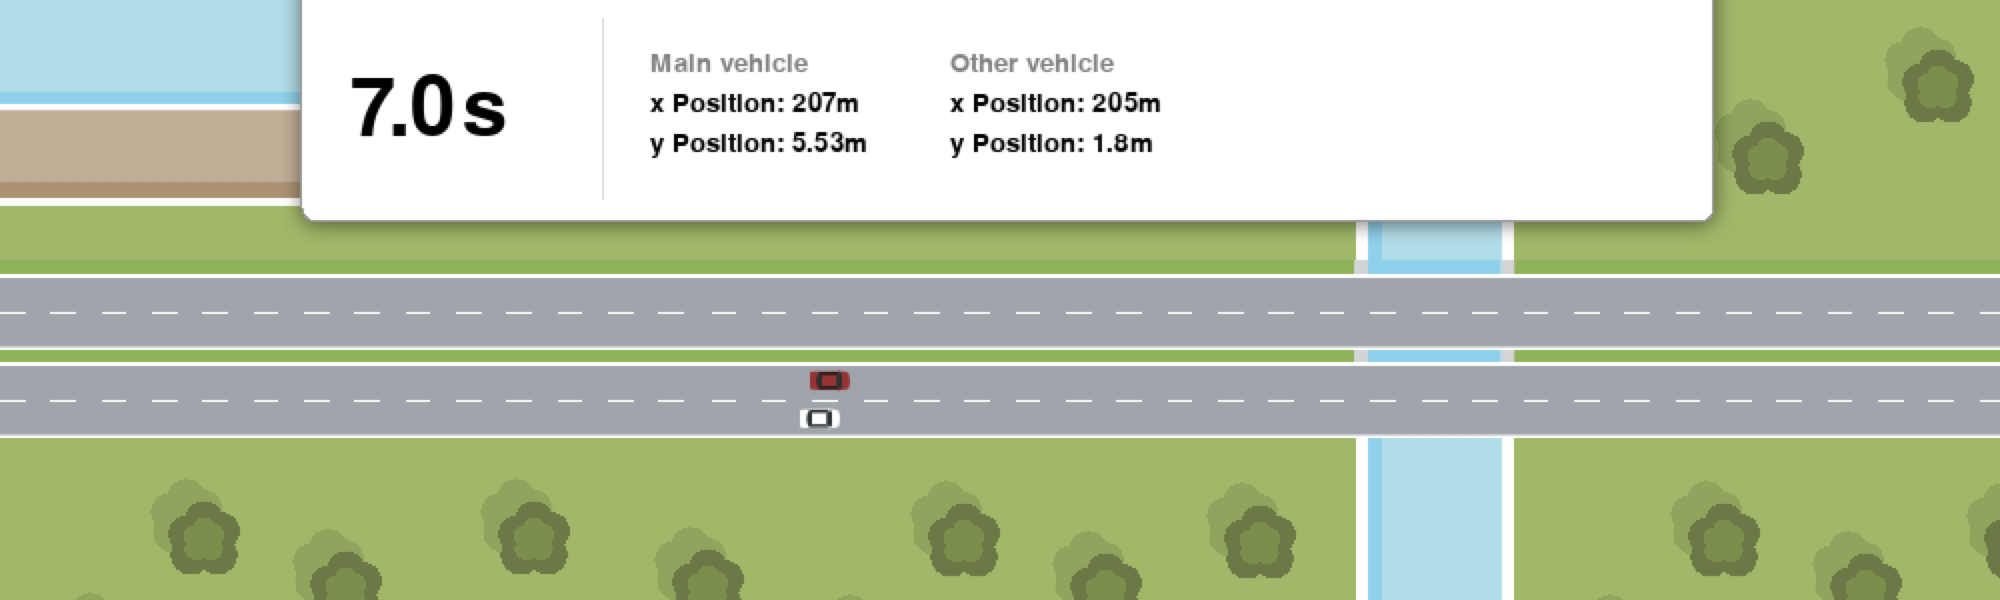
\includegraphics[width=1\linewidth]{snap_2.png}
\end{subfigure} \\ \vspace{2px}
\begin{subfigure}{0.75\textwidth}
  \centering
  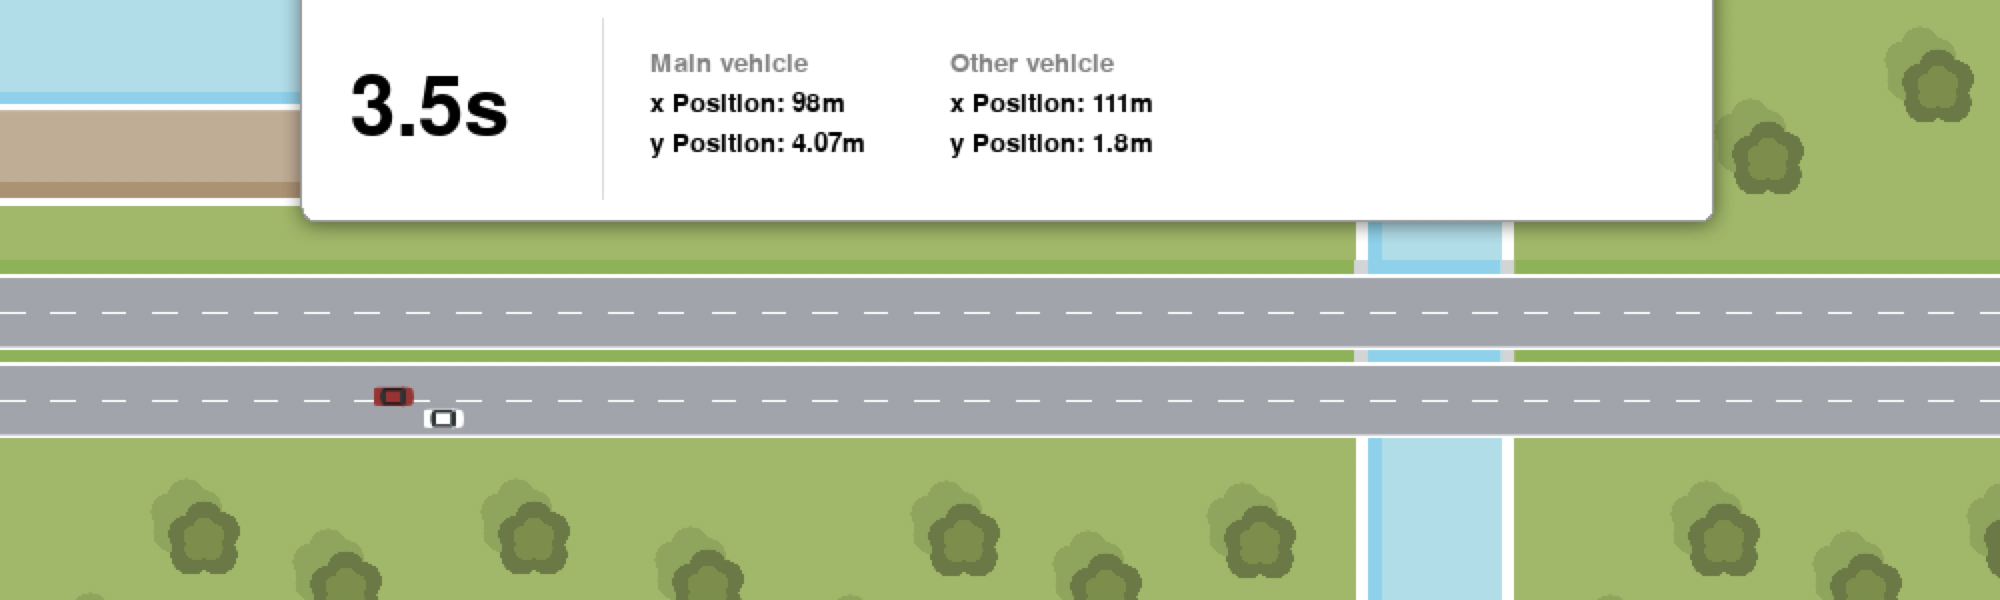
\includegraphics[width=1\linewidth]{snap_3.png}
\end{subfigure} \\ \vspace{2px}
\begin{subfigure}{0.75\textwidth}
  \centering
  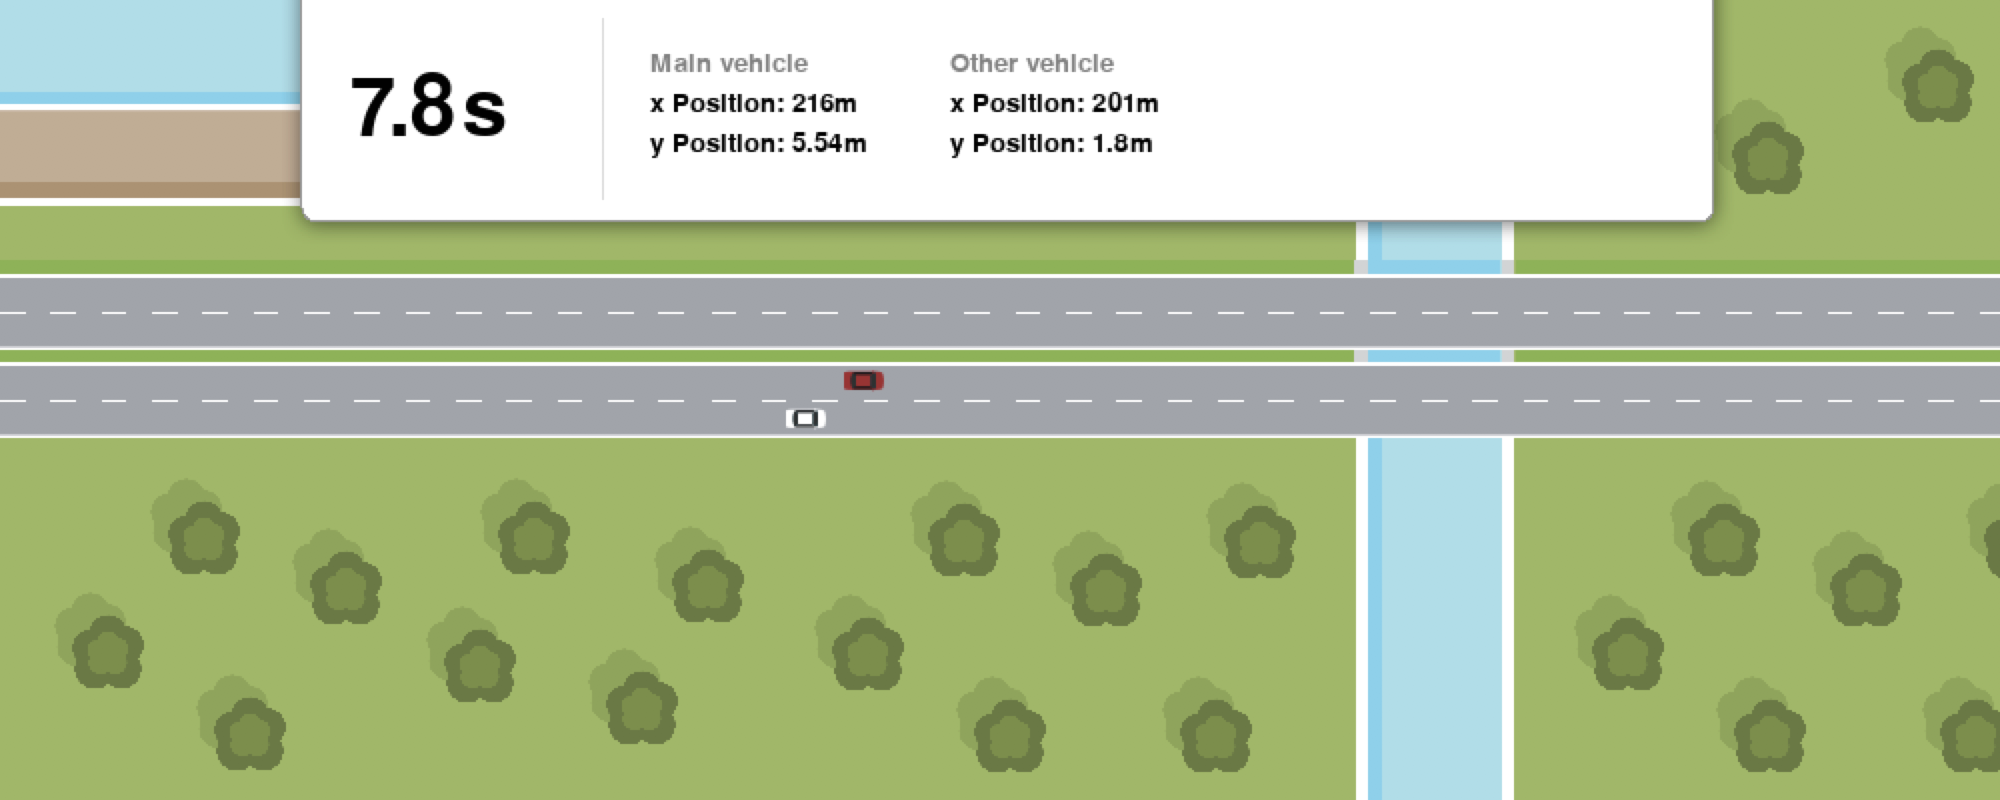
\includegraphics[width=1\linewidth]{snap_4.png}
\end{subfigure} \\ \vspace{2px}
\begin{subfigure}{0.75\textwidth}
  \centering
  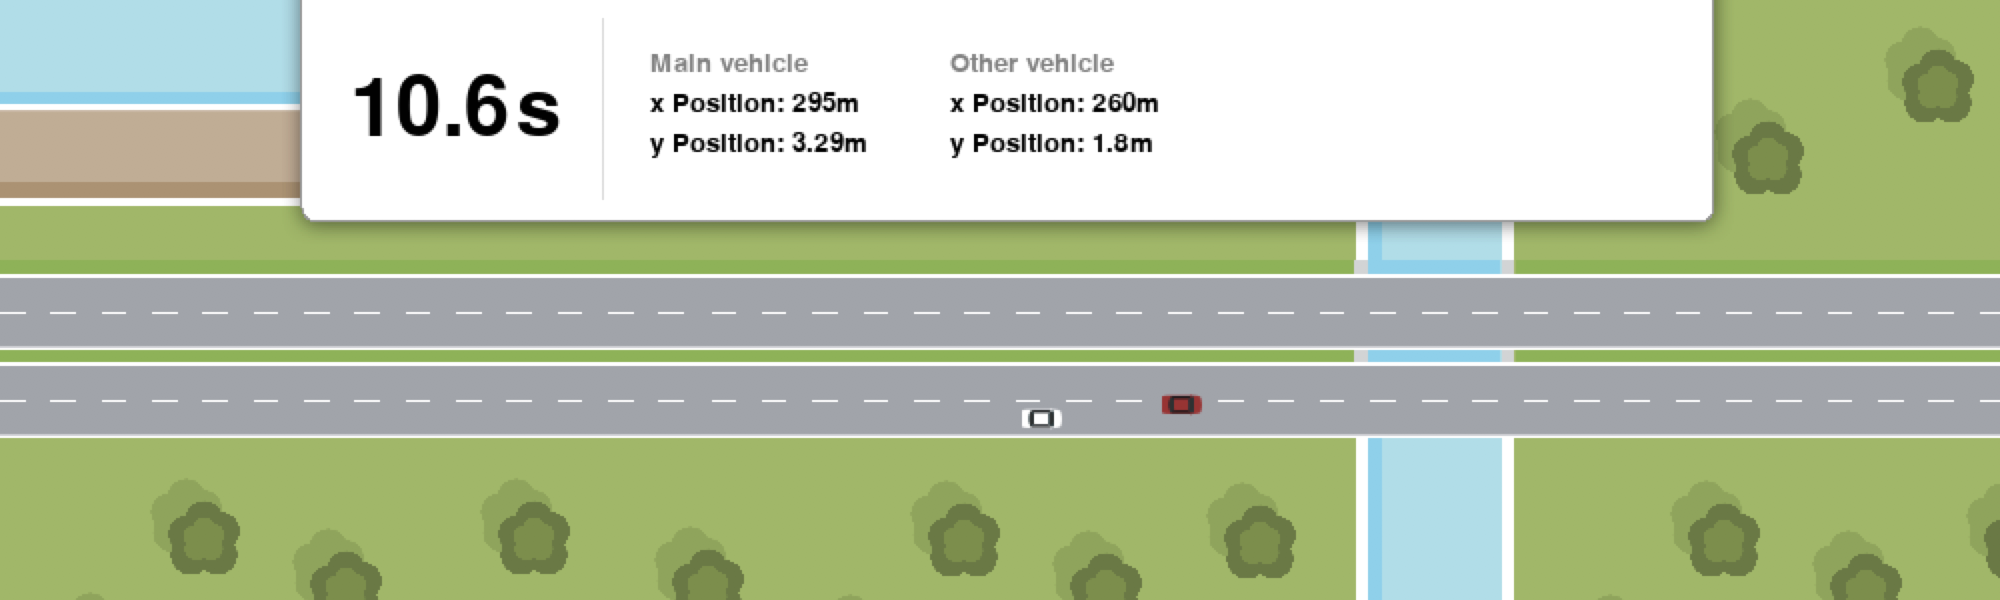
\includegraphics[width=1\linewidth]{snap_5.png}
\end{subfigure} \\ \vspace{2px}
\begin{subfigure}{0.75\textwidth}
  \centering
  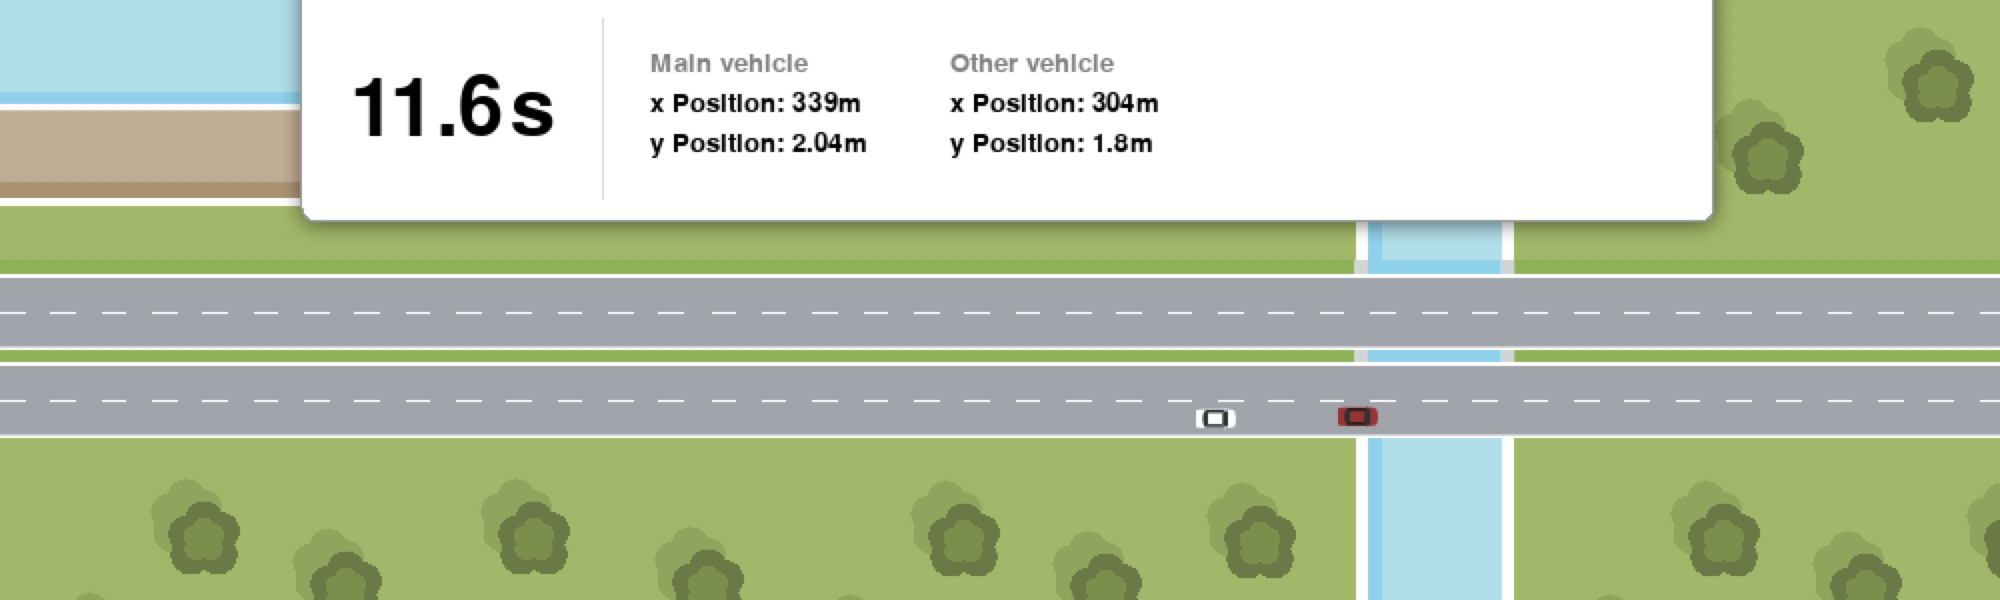
\includegraphics[width=1\linewidth]{snap_6.png}
\end{subfigure}
\caption{Snapshots of the simulator for one of the paths in the scenario $(d_{type}, v, v_1, x_{1,0}) = (3, 28, 21, 38)$.}
\label{fig:example_sim}
\end{figure}


